\RequirePackage{silence} % :-\
    \WarningFilter{scrbook}{Usage of package `titlesec'}
    \WarningFilter{titlesec}{Non standard sectioning command detected}
\documentclass[11pt,paper=b5,footinclude,headinclude]{scrbook} % KOMA-Script book
\usepackage[T1]{fontenc}
\usepackage[style=arsclassica, parts=false, eulermath=false, palatino=true, eulerchapternumbers=true]{classicthesis}


%\documentclass[11pt,a5paper,footinclude,headinclude]{scrbook} % KOMA-Script book

\usepackage{xspace,xcolor,afterpage}
\usepackage{url}
\usepackage{enumerate}
\usepackage{comment}
\usepackage{graphicx}
\usepackage{amsfonts,amsmath,amssymb,amsthm}
\usepackage{graphics}
\usepackage{color}
\usepackage{fullpage}
\usepackage{makecell}
%\usepackage{times}
%\usepackage{txfonts}
\def\P {{\cal P}}
\def\ali {{~\vee~}}
\def\inn {{~\wedge~}}
\def\sledi {{~\Rightarrow~}}
\def\brez {{\,\setminus\,}}
\def\cee {{~\Leftrightarrow~}}
\def\zgled{\paragraph{Example:}}
\def\kz{{\hfill{\S}}}% konec zgleda
\newenvironment{example}{\paragraph{Example:}}{\hfill \S}

\theoremstyle{remark}
\newtheorem*{remark}{Remark}
\newtheorem*{lemma}{Lemma}
\newtheorem*{corollary}{Corollary}
\theoremstyle{definition} %theorem
\newtheorem*{definition}{Definition}
\theoremstyle{theorem} %theorem
\newtheorem*{theorem}{Theorem}
\newtheorem*{proposition}{Proposition}

%vars
\newcommand{\myTitle}{Theoretical Computer Science\xspace}
\newcommand{\mySubtitle}{Discrete Structures for Computer Science Students \xspace} 				%dodaj podnaslov if needed
\newcommand{\myName}{UP FAMNIT \xspace}
\newcommand{\myPublisher}{Matjaž Krnc}
\newcommand{\myMonth}{Spring}
\newcommand{\myYear}{2021}
\newcommand{\verzija}{Version 0.1\xspace}
\newcommand{\shortAuthors}{M. Krnc}
\newcommand{\myAuthors}{Matjaž Krnc}
\newcommand{\myISBN}{978-961-XXX-XXX-X }
\newcommand{\myRepo}{\url{https://github.com/mkrnc/TOR1-vaje---TCS1-exercises.git}}


\begin{document}
%*******************************************************
% Titlepage
%*******************************************************
\begin{titlepage}
\definecolor{amber}{rgb}{1.0, 0.75, 0.0}
\pagecolor{amber}\afterpage{\nopagecolor}
	% if you want the titlepage to be centered, uncomment and fine-tune the line below (KOMA classes environment)
	\begin{addmargin}[-1cm]{-1cm}
    \begin{center}
        \large  

        \hfill

        \vfill

        \begingroup
            \color{Maroon}\spacedallcaps{\LARGE\myTitle} \\ \bigskip
        \endgroup

        \spacedlowsmallcaps{\mySubtitle}

        \vfill

        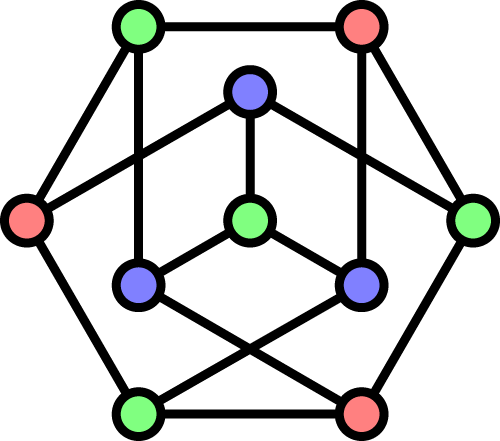
\includegraphics[width=11cm]{petersen.png} %\\ \medskip
				\vfill
        \myName \\ \medskip   
        %\myDegree \\
        %\myDepartment \\                            
        %\myFaculty \\
        %\myUni \\ \bigskip

        \myMonth \xspace \myYear \ -- \verzija

        \vfill                      

    \end{center}  
  \end{addmargin}       
\end{titlepage}   
%\begin{addmargin}[-1cm]{-1cm}
	{\vspace*{\fill}
	\setlength{\fboxsep}{6mm}
	\noindent\fbox{
	\begin{minipage}[b][6.5cm][c]{11cm} % velikost okvira škatle je 11 cm
							% x 6,5 cm
	\small
	CIP -- Katalo\v zni zapis o publikaciji\\
	Narodna in univerzitetna knji\v znica, Ljubljana
	
	\vfill

	123.4(567)(8.901.2)
	\vfill

	TEORETIČNE osnove računalništva -- vaje / avtor \shortAuthors; [urednik] M. Krnc. - \verzija.  - El. knjiga. - Ljubljana : samozal. M. Krnc, 2020.
	\vfill
	
	Način dostopa (URL):\\ \myRepo
	
	\vfill
	
	ISBN \myISBN  (pdf)\\
	%1. Milanič, Martin 2. Krnc, Matjaž, 1987-
	123456789
	\vfill
	
	\end{minipage}}}
%\end{addmargin}
\endinput
\newpage
\section*{Preface}
   

Those notes are supposed to be parsed together with explanations from the lectures.
Any questions or found errors should be 
addressed to \url{matjaz.krnc@upr.si}, or 
raised as an issue in our public repository 
\begin{center}
    \myRepo.    
\end{center}


Among most notable student contributors are:


\newpage
\vspace*{\fill}
\noindent

\begin{tabular}{ll}
%Lektorirala: ...\\[3mm]
\multicolumn{2}{ l }{\textbf{\myTitle}} \\
\multicolumn{2}{ l }{\emph{\mySubtitle}} \\[6mm]
\textbf{Authors:} & \parbox[t]{6cm}{\myAuthors \vspace{3mm}}\\
\textbf{Editor:} & Matjaž Krnc\\[3mm]
\textbf{Cover photo:} & \parbox[t]{6cm}{R. A. Nonenmacher\\ \emph{Desargues Graph} \vspace{3mm}}\\
\textbf{Design and self-publishing:} & \parbox[t]{6cm}{\myPublisher \vspace{3mm}}\\[6mm]
%\textbf{Oblikovanje:} & Matjaž Krnc\\[3mm]
\textbf{ISBN:} &  \myISBN \\
%Priprava za tisk: \\[3mm]
%Tisk: \\[3mm]
Ljubljana, \myMonth\xspace\myYear
\end{tabular}



\endinput

\tableofcontents


\chapter{Mathematical Logic}
{Those exercises are unfortunately in Slovene language. I still believe it may be of help to some of you. Also feel free to contribute translations!}
\begin{enumerate}
    \item 
    (Naloga o vitezih in oprodah)
A, B, C, D, E
\begin{itemize}
  \item A: ``D je oproda in C je oproda."
  \item B: ``Če sta A in D oprodi, potem je C oproda."
  \item C: ``Če je B oproda, potem je A vitez."
  \item D: ``Če je E oproda, potem sta C in B oprodi."
\end{itemize}

\medskip
\textbf{Rešitev:}

Naj bo $A$ izjava: ``A je vitez", itd.
Iščemo tisto edino določilo $d$, za katerega je izjava $$A_1\inn B_1\inn C_1\inn D_1$$
pravilna, kjer je:

$A_1: A\cee (\neg D \inn \neg C)$

$B_1: B\cee (\neg A \inn \neg D\sledi \neg C)$

$C_1: C\cee (\neg B \sledi A)$

$D_1: D\cee (\neg E \sledi \neg C \inn \neg B)$


Ker bi pravilnostna tabela vsebovala 32 vrstic, rešimo nalogo
raje z analizo primerov.

\textbf{1.~primer: $A(d) = 1$.}
Zaradi $A_1$ je potem $D(d) = 0$ in $C(d) = 0$.

V izjavo $C_1$ vstavimo $A(d) = 1$ in $C(d) = 0$, dobimo:
$\neg(\neg B\sledi 1)$,

$\neg(B\ali 1)$,

$\neg 1$, to pa je nepravilna izjava.

Torej 1.~primer ni mogoč.
%
% torej $B(d) = 1$.
%
%V izjavo $B_1$ vstavimo $A(d) = 1$, $B(d) = 1$, $C(d) = 0$ in $D(d) = 0$, dobimo:
%$1\cee (0\inn 1\sledi 1)$, kar je pravilna izjava.
%
%V izjavo $D_1$ vstavimo znane vrednosti, dobimo:
%$\neg(\neg E \sledi 1 \inn 0)$
%
%$\neg(\neg E \sledi 0)$
%
%Sledi $\neg E(d) = 1$, torej $E(d) = 0$.
%

\textbf{2.~primer: $A(d) = 0$.}

Zaradi $A_1$ je bodisi $C(d) = 1$ ali pa $D(d) = 1$.

\textbf{2.1.: $C(d) = 1$}.

Zaradi $C_1$ je $\neg B \sledi 0$, torej je $\neg B = 0$ in posledično $B(d) = 1$.

V izjavo $B_1$ vstavimo $A(d) = 0$, $B(d) = 1$, $C(d) = 1$, dobimo:

$1 \inn \neg D\sledi 0$

$\neg D\sledi 0$

Sledi $\neg D = 0$ oz.~$D(d) = 1$.

Vstavimo v izjavo $D_1$ znane vrednosti:

$(\neg E \sledi 0 \inn 0)$

Sledi $E(d) = 1$.

\bigskip

\textbf{2.2.: $C(d) = 0$ in $D(d) = 1$}.

Iz izjave $B_1$ dobimo $B(d) = 1$.

Izjava $C_1$ pa je sedaj nepravilna:
$0 \cee (0\sledi 1)$.\qed

Torej so $B$, $C$, $D$ in $E$ vitezi, $A$ pa je oproda.


\bigskip
\item (Sklepanje)
Ali je naslednje sklepanje pravilno?

Mislim, torej sem. Mislim, torej sklepam. Sklep: Sem, torej sklepam.


\textbf{Rešitev:}

$A_1$: Mislim.

$A_2$: Sem.

$A_3$: Sklepam.

Zanima nas pravilnost implikacije

$$(A_1\sledi A_2)\inn(A_1\sledi A_3)\sledi(A_2\sledi A_3)$$

Pri določilu $A_1(d) = 0$, $A_2(d) = 1$, $A_3(d) = 0$ je ta implikacija nepravilna!
(Ne mislim, sem, ne sklepam.)
Torej je sklepanje napačno.

\bigskip

\item (Sklepanje)
Ali je naslednje sklepanje pravilno?

Dojenčki se obnašajo nelogično. Kdor je sposoben ukrotiti krokodila, je spoštovanja vreden.
Kdor se obnaša nelogično, ni spoštovanja vreden. Sklep: Dojenčki niso sposobni ukrotiti krokodila.


\textbf{Rešitev:}

$A_1$: Sem dojenček.

$A_2$: Obnašam se nelogično.

$A_3$: Sposoben sem ukrotiti krokodila.

$A_4$: Vreden sem spoštovanja.

$(A_1\sledi A_2)\inn (A_3\sledi A_4) \inn (A_2\sledi \neg A_4)\sledi (A_1\sledi \neg A_3)$

Pa recimo, da je sklep napačen. Tedaj obstaja določilo $d$, da velja
\begin{enumerate}[(1)]
  \item $(A_1(d)\sledi \neg A_3(d)) = 0$
  \item $(A_1(d)\sledi A_2(d)) = 1$
  \item $(A_3(d)\sledi A_4(d)) = 1$
  \item $(A_2(d)\sledi \neg A_4(d)) = 1$
\end{enumerate}
Torej je, zaradi (1), $A_1(d) = 1$ in $A_3(d) = 1$. Zaradi (2) je $A_2(d) = 1$.
Zaradi (4) je $A_4(d) = 0$. To pa je protislovje s (3).

Torej je sklepanje pravilno.\qed

% 8. in 9. predavanje, 4 ure (Istvan), 7. in 8. 11. 2012

%\bigskip
%Rešitev domače naloge:
%
%Dejstva:
%
%Barona je umoril eden izmed njegovega osebja: kuharica, strežnik ali šofer.
%
%Če je morilka kuharica, je zastrupila hrano.
%
%Če je morilec šofer, mu je postavil bombo v avto.
%
%Hrana ni bila zastrupljena in strežnik ni morilec.
%
%Sklep: Morilec je šofer.
%
%\bigskip
%
%\textbf{ Rešitev:}
%
%$K$: Morilka je kuharica.
%
%$S$: Morilec je strežnik.
%
%Š: Morilec je šofer.
%
%H: Kuharica je zastrupila hrano.
%
%B: Šofer je postavil bombo v avto.
%
%\medskip
%Ali je naslednja implikacija tavtologija?
%
%$(K\ali S\ali$ \v S$)\inn(K\sledi H)\inn($Š$\sledi B)\inn(\neg H\inn \neg S)\sledi $Š
%
%\bigskip
%Recimo, da ni.
%
%(1) $(K\ali S\ali$ \v S$)(d) = 1$
%
%(2) $(K\sledi H)(d) = 1$
%
%(3) (Š$\sledi B)(d) = 1$
%
%(4) $(\neg H\inn \neg S)(d) = 1$
%
%(5) Š$(d) = 0$
%
%Iz (4) sledi:
%
%(5)  $H(d) = S(d) = 0$.
%
%Iz (2) in (5) potem sledi
%
%(6) $K(d) = 0$.
%
%Iz (1), (5) in (6) potem sledi Š$(d) = 1$. Protislovje. Izjava je tavtologija  in sklepanje je pravilno.
%


\item
The following two propositions are given:
$A$: ``Andrej speaks French.'' and $B$: ``Andrej speaks Danish.''
Write the following compound propositions in natural language:

(a) $A\ali B$

(b) $A\inn B$

(c) $A\inn \neg B$

(d) $\neg A\ali \neg B$

(e) $\neg \neg A$

(f) $\neg (\neg A\inn \neg B)$

\medskip
\item
The following two propositions are given:
$A$: ``Janez is rich.'' and $B$: ``Janez is happy.''

Write the following propositions symbolically:

(a) If Janez is rich, then he is unhappy.

(b) Janez is neither happy nor rich.

(c) Janez is happy only if he is poor.

(d) Janez is poor if and only if he is unhappy.

\item Solve the following exercises about knights and servants:
\begin{itemize}
  \item Arthur: ``It is not true that Bine is a servant."~Bine: ``We are not both of the same kind.''
  \item Arthur: ``It is not true that Cene is servant."~Bine: ``Cene is a knight or I am a knight."~Cene: ``Bine is a servant."
\end{itemize}

\item {A similar exercise:}
Now Arthur and Bine say the following:
\begin{itemize}
 \item Arthur: ``Me and Bine are not of the same kind.''
 \item Bine: ``Exactly one of us is a knight.''
\end{itemize}
\item Given the propositions:\\
$A:$ ``It's cold outside''\\
$B:$ ``It's raining''\\
express the following propositions in natural language:
\begin{enumerate}
\item $\neg A$
\item $A\wedge B$
\item $A\vee B$
\item $B\vee\neg A$
\end{enumerate}
\item Given the propositions:\\
$A:$ ``John reads The New York Times.''\\
$B:$ ``John reads The Wall Street Journal.''\\
$C:$ ``John reads The Daily Mail.''\\
\\
Transcribe the following statements into symbolic propositions:
\begin{enumerate}
\item John reads The New York Times, but not The Wall Street Journal.
\item Either John reads both The New York Times and The Wall Street Journal,
or he does not read The New York Times and The Wall Street Journal.
\item It is not true that John reads The New York Times, and does not read
The Daily Mail.
\item It is not true that John reads The Daily Mail or The Wall Street Journal,
and not The New York Times.
\end{enumerate}
\item Find the truth tables for the symbolic propositions from (2).
\begin{enumerate}
\item For three lines $p,q,r$ we may construct also geometric propositions.
Suppose that the following is true:
\[
(p||q)\wedge(p\cap q\neq\emptyset)\wedge(q\cap r\neq\emptyset).
\]
What can you ay about the lines $p,q,r$?
\end{enumerate}
\item Knights and servants! For both cases below (separately) determine
the roles.
\begin{enumerate}
\item Arthur: It's not true that Chloe is a servant.\\
Bob: Chloe is a knight, or I am a knight.\\
Chloe: Bob is a servant.
\item Arthur: Chloe or Bob are servants.\\
Bob: Cene and Arthur are knights.
\end{enumerate}
\item Express the propositions below with connectives $\wedge$ and $\neg$
only!
\begin{enumerate}
\item $A\vee B$
\item $A\Rightarrow B$
\item $A\Leftrightarrow B$
\end{enumerate}


\item Find the canonical disjunctive normal form (DNF) and the canonical conjuctive normal form (CNF) for the following propositions:
\begin{enumerate}
\item[(i)] $\neg(A\wedge B) \Rightarrow (\neg B \Rightarrow A)$
\item[(ii)] $\neg (A\vee B) \wedge (A \Rightarrow B)$
\end{enumerate}

\emph{Rešitev.} (i) Napiši pravilnostno tabelo. DNO: vzemi vrstice z enicami (poveži jih med sabo s konjunkcijo) in jih poveži med sabo z disjunkcijo
$(A\wedge B) \vee (A\wedge \neg B) \vee (\neg A \wedge B)$. KNO: vzemi vrstice z ničlami (vzemi nasprotne vrednosti in jih poveži med sabo z disjunkcijo) in jih poveži med sabo s konjunkcijo $(A \vee B)$. (ii) Podobno.

\item For the following compound proposition find  a truth table, determine DNF, CNF and draw the corresponding circuit.
$$
(A \Rightarrow (B\Rightarrow C)) \Rightarrow ((A\Rightarrow B)\Rightarrow (A \Rightarrow C)).
$$


\item Find a compound proposition $\mathcal{I}$ such that
$$(A\Rightarrow (\mathcal{I} \Rightarrow \neg B))\Rightarrow (A\wedge B) \vee \mathcal{I}$$
is tautology.

\emph{Rešitev.} Napiši pravilnostno tabelo za osnovni izjave $A, B$ skupaj s (sestavljeno) izjavo $\mathcal{I}$. Iz nje razberi, da je pravilnostna tabela za $\mathcal{I}$ enaka
\begin{table}[ht!]
\centering
\begin{tabular}{c|c|c}
A & B & $\mathcal{I}$\\
\hline
1 & 1 & 0\\
1 & 0 & 1\\
0 & 1 & 1\\
0 & 0 & 1
\end{tabular}
\end{table}

Torej je $\mathcal{I} \Leftrightarrow \neg A \vee \neg B$ v KNO.
\pagebreak

\item For the following circuits find the  corresponding compound propositions

\noindent (i)
\begin{center}
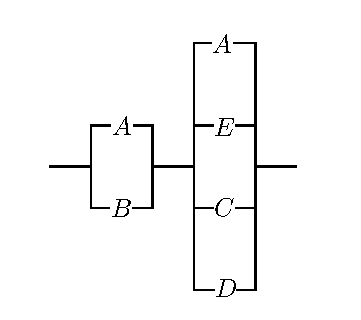
\includegraphics{img/vez1}
\end{center}
\noindent (ii)
\begin{center}
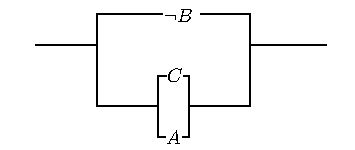
\includegraphics{img/vez2}
\end{center}
\noindent (iii)
\begin{center}
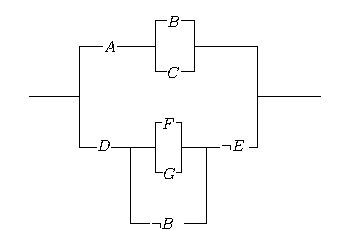
\includegraphics{img/vez3}
\end{center}




\item Simplify the following logical equivalence
$$(A\Rightarrow B) \vee (B \Rightarrow C).$$

\emph{Rešitev.} 
\begin{eqnarray*}
(A\Rightarrow B) \vee (B \Rightarrow C) &\Leftrightarrow & (\neg A \vee B) \vee (\neg B \vee C)\\
&\Leftrightarrow & \neg A \vee B \vee \neg B \vee C\\
&\Leftrightarrow & \neg A \vee (B \vee \neg B) \vee C\\
&\Leftrightarrow & \neg A \vee 1 \vee C\\
&\Leftrightarrow & 1.
\end{eqnarray*}

\item Show that the following propositions are logical implications (a tautology where the main connective is implication).
\begin{enumerate}
\item[(i)] $A \wedge (A \Rightarrow B) \Rightarrow B$
\item[(ii)] $\neg B \wedge (A \Rightarrow B) \Rightarrow \neg A$
\item[(iii)] $\neg A \wedge (A \vee B) \Rightarrow B$
\item[(iv)] $(A \Rightarrow B) \wedge (B \Rightarrow C) \Rightarrow (A \Rightarrow C)$
\item[(v)] $A \wedge (A \Leftrightarrow B) \Rightarrow B$
\end{enumerate}

\emph{Rešitev.} (i) Recimo $A \wedge (A \Rightarrow B)$ pravilna, $B$ pa nepravilna. Potem je $A$ pravilna in $A\Rightarrow B$ pravilna. Sledi $B$ pravilna. Protislovje. 


\item Are the following propositions logical implications?
\begin{enumerate}
\item[(i)] $(A \Rightarrow B ) \wedge (A \Rightarrow C) \wedge A \Rightarrow B \wedge C$
\item[(ii)] $\neg (A \vee B) \wedge (A\vee C) \wedge (D\Rightarrow C) \Rightarrow D$
\item[(iii)] $(A\Rightarrow B) \wedge (A\Rightarrow C) \wedge (D\wedge E \Rightarrow F) \wedge (C\Rightarrow E) \Rightarrow F$
\end{enumerate}

\item With a direct proof show:
\begin{quote}
    If $n$ is even, then so is $n^2 +3n$.
\end{quote}
Is the converse also true?

%Z direktnim dokazom implikacije pokaži: Če je $n$ sodo število, potem je $n^2 +3n$ sodo. Ali je obrat pravilen? 

\item Z direktnim dokazom implikacije pokaži: Če je realno število $x$ nenegtivno, potem je vsota  števila $x$  in njegove obratne vrednosti  večja ali enaka $2$.


\emph{ Rešitev.} Pokažimo $x + \frac{1}{x}\geq 2$. Ker $x\geq 0$, pomnožimo neenakost z $x$ in dobimo
$x^2 + 1 \geq 2x$ oziroma $(x- 1)^2\geq 0$. Slednje je očitno vedno res.

\item S protislovjem pokaži, da je praštevil neskončno.

\emph{ Rešitev.} Recimo, da jih je končno mnogo $p_1,p_2,\ldots, p_n$. Potem  $p=p_1p_2\cdots p_n+1$ ni deljivo z nobenim praštevilom $p_i$ in $p_i\neq p$ za vsak $i$. Po definiciji je torej $p$ praštevilo, ki ni enako nobenemu prejšnjemu. Protislovje.

\item Poišči napako v naslednjem dokazu. 

\textbf{Trditev:} $1$ je največje naravno število. 

\textbf{Dokaz} (s protislovjem):
Predpostavimo nasprotno. Naj bo $n>1$ največje naravno število. Ker je $n$ pozitivno, lahko neenakost $n>1$ pomnožimo z $n$. Torej $n>1\Leftrightarrow n^2>n$. Dobili smo, da je $n^2$ večje od $n$, kar je v protislovju s predpostavko, da je $n$ največje naravno število. Torej je bila predpostavka napačna in je $1$ največje naravno število.

\emph{ Rešitev.} Nasporotna trdtev je: obstaja naravno število, ki je večje od $1$.


\item Let  $x$ and $y$ be real numbers such that $x<2y$. 
By an indirect proof show: 
\begin{quote}
    If $7xy\leq 3x^2 + 2y^2$, then $3x\leq y$.
\end{quote}

\emph{ Solution (in slovene).} Naj bo $x<2y$, to je, $2y-x>0$. Pokazali bomo: če je $3x> y$, potem je $7xy > 3x^2 + 2y^2$. Predpostavimo torej, da je $3x-y>0$. Potem je $(2y-x)(3x-y)= 7xy - 3x^2 - 2y^2>0$, to je, $7xy > 3x^2 + 2y^2$.

\item Dokaži naslednjo ekvivalenco v dveh delih: Naj bosta $m$ in $n$ celi števili. Tedaj sta števili $m$ in $n$ različnih parnosti natanko tedaj, ko je število $m^2- n^2$ liho.

\emph{ Rešitev.} ($\Rightarrow$) Predpostavimo, da sta različnih parnosti. Pišimo  $m=2k$ in $n=2l+1$, vstavimo v izraz $m^2- n^2$ in rezultat sledi.

($\Leftarrow$) Pokažemo indirektno in sicer: Če sta $m$ in $n$ iste parnosti, potem je $m^2- n^2$ sodo. Obravnavaj oba primera.


\item Z uporabo če in samo če dokaza pokaži: $ac\,|\,bc \Leftrightarrow a\,|\,b$.

\item Ali je naslednji sklep pravilen?
\begin{enumerate}
\item[(i)] Če je danes sreda bom imel vaje. Danes je sreda. Sklep: Imel bom vaje.

\emph{ Rešitev.} $(A\Rightarrow B) \wedge A \Rightarrow B$. Res je.

\item[(ii)] Če se učim, bom opravil izpit. Nisem se učil. Sklep: Ne bom opravil izpita.

\emph{ Rešitev.} $(A\Rightarrow B) \wedge \neg A \Rightarrow \neg B$. Ni nujno res.
\end{enumerate}

\item Ali je naslednji premislek pravilen?
\begin{enumerate}
\item[(i)] Študent se je z mestni avtobusom odpravil na izpit. Rekel si je: Če bo na naslednjem semaforju zelena luč, bom naredil izpit. No, ko je avtobus pripeljal na naslednji semafor, na semaforju ni svetila zelena luč, študent pa si je dejal: Presneto, spet bom padel.

\emph{ Rešitev.} $((A\Rightarrow B) \wedge \neg A) \Rightarrow \neg B$. Ni nujno res.

\item[(ii)] Inženir, ki obvlada teorijo, vedno načrta dobro vezje. Dobro vezje je ekonomično. Torej, inženir, ki načrta neekonomično vezje, ne obvlada teorije. 

\emph{ Rešitev.} $((A\Rightarrow B) \wedge (B\Rightarrow C)) \Rightarrow (\neg C \Rightarrow \neg A)$. Res je.
\end{enumerate}





\item Which of the following propositions are correct where the language of the conversation are real numbers?
\begin{enumerate}
\item[(i)] $(\forall x)(\exists y)(x+y=0)$.
\item[(ii)] $(\exists x)(\forall y)(x+y=0)$.
\item[(iii)] $(\exists x)(\exists y)(x^2+y^2 =-1)$.
\item[(iv)] $(\forall x)[x>0 \Rightarrow (\exists y)(y<0 \wedge xy>0)]$.
\end{enumerate} 
\end{enumerate} 

\chapter{Set theory}
\begin{enumerate}

\item Let $A = \{ x \in \mathbb{N}; x < 7\}, B = \{x \in  \mathbb{Z}; |x - 2| < 4\}$ and $C = \{x \in\mathbb{R}; x^3 -  4x = 0\}$.
\begin{enumerate}
\item[(i)]  Write down the elements for all three sets.
\item[(ii)] Find $A \cup C, B \cap C, B \setminus C, (A \setminus B) \setminus C$ and $A \setminus (B \setminus C)$.
\end{enumerate}

\item Let  $\mathbb{Z}$ be a universal set and let  $P$ denote the set of all prime numbers, and $S$ the set of all even integers. Write the following propositions in terms of set theory:
\begin{itemize}
\item[(i)] There exists an even prime number. \quad [$P\cap S \neq \emptyset$]
\item[(ii)] $0$ is an integer, but it is not natural number. \quad [$0 \in \mathbb{Z}\setminus \mathbb{N}$]
\item[(iii)] Every natural number is an integer. \quad [$\mathbb{N}\subseteq \mathbb{Z}$]
\item[(iv)] Not every integer is a natural number. \quad [$\mathbb{Z}\nsubseteq \mathbb{N}$]
\item[(v)] Every prime number except 2 is odd. \quad [$P\setminus \{2\} \subseteq \overline{S}$]
\item[(vi)] 2 is an even prime number. \quad [$2\in S\cap P$]
\end{itemize}

\item Let  $A, B, C$ and $D$  be subsets of some universal set  $U$. Simplify the following expression
$$\overline{(\overline{(A\cup B)} \cap \overline{(\overline{A} \cup C)})}\setminus \overline{D}.$$

\item Show that $(A\cup C)\cap (B\setminus C) = (A\cap B)\setminus C$.

\emph{ Rešitev.} 
\begin{eqnarray*}
x\in (A\cup C)\cap (B\setminus C) &\Leftrightarrow & (x\in A \vee x\in C) \wedge (x\in B \wedge x\notin C)\\
 &\Leftrightarrow & ((x\in A \vee x\in C) \wedge (x\notin C))\wedge x\notin B\\
&\Leftrightarrow & ((x\in A \wedge x\notin C) \vee (x\in C \wedge x\notin C)) \wedge
 x\in B\\
&\Leftrightarrow & x\in A \wedge x\notin C  \wedge x\in B\\
&\Leftrightarrow & x\in A \wedge x\in B  \wedge x\notin C \\
&\Leftrightarrow & x \in (A\cap B)\setminus C. 
\end{eqnarray*}

\item (Zadnja lastnost pri uniji) Prove that $A\subseteq C  \wedge B\subseteq C \Rightarrow A\cup B\subseteq C$.

\emph{ Rešitev.} Direktno.

\item (Predzadnja lastnost pri preseku) Prove that $A\subseteq  B \Leftrightarrow A\cap B = A$.

\emph{ Rešitev.} V dveh delih.

\item (Predzadnja lastnost pri kartezičnemu produktu) Prove that $A\times (B\cap C) = (A\times B)\cap (A\times C)$.

\emph{ Rešitev.} 
\begin{eqnarray*}
(x,y)\in A\times (B\cap C) &\Leftrightarrow & x \in A \wedge y\in B\cap C\\
&\Leftrightarrow & x \in A \wedge y\in B  \wedge y\in C\\
&\Leftrightarrow & x \in A \wedge x \in A\wedge y\in B  \wedge y\in C\\
&\Leftrightarrow & x \in A \wedge  y\in B  \wedge x \in A\wedge y\in C\\
&\Leftrightarrow & (x,y) \in A\times B \wedge  (x,y) \in A\times C\\
&\Leftrightarrow & (x,y) \in (A\times B)\cap   (A\times C).
\end{eqnarray*}

\item (Predzadnja lastnost pri razliki) Prove that $(A\cap B )\setminus B = \emptyset$.
\emph{ Rešitev.} 
\begin{eqnarray*}
x\in (A\cap B )\setminus B  &\Leftrightarrow & x \in (A\cap B)  \wedge x\notin B\\
&\Leftrightarrow & (x\in A\wedge x\in  B ) \wedge x\notin B\\
&\Leftrightarrow & x\in A\wedge (x\in  B  \wedge x\notin B)\\
&\Leftrightarrow & x\in \emptyset.
\end{eqnarray*}

\item Determine the following sets:
\begin{enumerate}
\item[(i)] $\{\emptyset, \{\emptyset\}\}\setminus \emptyset$ \quad [$\{\emptyset, \{\emptyset\}\}$]
\item[(ii)] $\{\emptyset, \{\emptyset\}\}\setminus \{\emptyset\}$
\item[(iii)] $\{\emptyset, \{\emptyset\}\}\setminus \{\}\emptyset\}\}$
\item[(iv)] $\{1,2,3,\{1\}, \{5\}  \}\setminus \{2,\{3\},5\}$
\end{enumerate}

\item Which of the following propositions are correct for arbitrary sets $A, B$ and $C$:
\begin{enumerate}
\item If $A\in B$ and $B\in C$, then $A\in C$.
\item If $A\subseteq B$ and $B\in C$, then $A\in C$.
\item If $A\cap B\subseteq \overline{C}$ and $A\cup C \subseteq B$, then $A\cap C = \emptyset$.
\item If $A\neq B$ and $B\neq C$, then $A\neq C$.
\item If $A\subseteq \overline{(B\cup C)}$ and $B\subseteq \overline{(A\cup C)}$, then $B=\emptyset$.
\end{enumerate}

\emph{ Rešitev.}
\begin{enumerate}
\item Napačna. Vzemi $A=\emptyset$, $B=\{\emptyset\}$, $B=\{\{\emptyset\}\}$.
\item Napačna. Vzemi isti primer kot v (a).
\item Pravilna. Dokaz s protislovjem. Recimo, da trditev ni pravilna. Naj bo $A\cap B\subseteq \overline{C}$, $A\cup C\subseteq B$  in naj obstaja $x\in A\cap C$. Torej je $x\in A$ in $x\in C$. Ker je po drugi predpostavki $A\cup C\subseteq B$, je $x\in B$. Sledi $x\in A \cap B$. Ker je po prvi predpostavki $A\cap B\subseteq \overline{C}$, je $x\in \overline{C}$. Protislovje, saj $x\in C$. 
\item Napačna. Vzemi $A=C\neq B$.
\item Napačna. Vzemi tri paroma disjunktne neprazne množice.
\end{enumerate}

\item Find $\mathcal{P}(A)$, where $A=\{a,b,c,d\}$.

\item Let $A=\{\{1,2,3\}, \{4,5\}, \{6,7,8\}\}$.
\begin{enumerate}
\item[(i)] Write down the elements of  $A$.
\item[(ii)] Is it true?\\
 (a) $1\in A$ \quad (b) $\{1,2,3\}\subseteq A$ \quad (c)  $\{6,7,8\}\in  A$ \quad  (d)  $\{\{4,5\}\}\subseteq A$\\
  (e) $\emptyset\in A$ \quad(f) $\emptyset\subseteq A$
\end{enumerate}


\item  Show that $A\times (B\cap C) = (A\times B)\cap (A\times C)$.



\item Let $A, B$ in $C$ be arbitrary subsets of the universal set $U= A \cup B \cup C$. Show the following propositions:
\begin{enumerate}
\item  $A\setminus B \subseteq \overline{B}$.
\item  $(A\setminus B)\cap B = \emptyset $.
\item  $A\cap B \subseteq C \Leftrightarrow A\subseteq \overline{B} \cup C$.
\item  $(A\setminus B) \cup B = A \Leftrightarrow B \subseteq A$.
\item  If $B\subseteq A$, then$B\times B = (B\times A)\cap (A\times B)$.
\item Let $A$ be a nonempty set. Which of the following sets 
$$\emptyset,\{\emptyset\}, A, \{A\}, \{A,\emptyset\}$$
are elements and which are subsets of (i) $\mathcal{P}(A)$ and (ii) $\mathcal{P}(\mathcal{P}(A))$?
\item  Is it true that  $\mathcal{P}(A\times B) = \mathcal{P}(A) \times \mathcal{P}(B)$?
\end{enumerate}


\end{enumerate}



\chapter{Relations}

\begin{enumerate}


\item Let $S=\{1,2,3,4,5\}$. 
\begin{enumerate}
    \item Is $R=\{(1,2),(2,3), (3,5), (2,4), (5,1)\}$ a binary relation?
    \item Find the domain $\mathcal{D} R$ and the range $\mathcal{Z} R$ of $R$.
    \item 
  Determine the inverse relation $R^{-1}$ and  $\mathcal{D} R^{-1}$ and  $\mathcal{Z} R^{-1}$.
\end{enumerate}

\item Let $R=\{(1,1),(2,1), (3,3), (1,5)\}$  and $T=\{(1,4),(2,1), (2,2), (2,5)\}$ be binary relations. \begin{enumerate}
    \item 
Determine the compositions $R\circ T$ and $T\circ R$. 
\item Is it true that $R\circ T = T \circ R$?
\end{enumerate}

\item Let  $S=\{1,2,3,4,5,6,7\}$. Define
$$R= \{(x,y)\,|\, x-y \textrm{ is divisible by  }  3\} \quad \mathrm{ in } \quad  T= \{(x,y)\,|\, x-y \geq 3\}.$$
Determine $R,T, R\circ R$.


\item Let  $S= \mathbb{R}$. On $S$ we define the relation $R$ as follows
$$(\forall x)(\forall y)(x R y \Leftrightarrow y \geq x +3).$$
Is $R$ reflexive, symmetric, transitive or strict total?

\item Let  $S=\{1,2,3,4\}$. We have the following relations
\begin{enumerate}
\item[(i)] $R_1= \{(1,1),(1,2),(2,3), (1,3), (4,4)\}$,
\item[(ii)] $R_2= \{(1,1),(1,2),(2,1), (2,2), (3,3), (4,4)\}$,
\item[(iii)] $R_3= \{(1,3),(2,1)\}$,
\item[(iv)] $R_4= \emptyset$,
\item[(v)] $R_5= S\times S$.
\end{enumerate}
Which of the following properties hold for each relation: reflexive, symmetric, antisymmetric, transitive?

\item Let $R$ and $S$ be symmetric relations. Show: $R\circ S$ symmetric $\Leftrightarrow R\circ S = S \circ R$.

\item Let $S= \{m\in \mathbb{N}\,|\, 1\leq n \leq 10\}$ in $R=\{(m,n)\in S\times S\,|\, 3|m-n\}$.
Is $R$ an equivalence relation? If yes, determine the corresponding equivalence classes and the factor set.

\section{Equivalences}
\item Let $S = \mathbb{Z}\times \mathbb{Z}$ and define the relation $R$ as follows
$$(a,b)R(c,d)\Leftrightarrow ad = bc.$$
Show that $R$ is an equivalence relation  and find the corresponding equivalence classes.

\item Let  $S =  \mathbb{R}^2$ and define the relation $R$ as follows
$$(x_1,y_1)R(x_2,y_2)\Leftrightarrow x_1^2 + y_1^2 = x_2^2 + y_2^2.$$
Show that $R$ is an equivalence relation  and find the equivalenec class $R[(7,1)]$.



\end{enumerate}
\section{Functions}
\begin{enumerate}

\item Let $A = \{1,2,3,4\}$, $B = \{x,y,z\}$, $C = \{a,b\}$. You are given functions $f:A\to B$ and $g:B\to C$.

\[ f = \{(1,x),(2,y),(3,y),(4,x)\} \]

\[ g = \{(x,a),(y,b),(z,b)\} \]

(a) Is $f$ injective?

(b) Is $f$ surjective?

(c) Is $g$ injective?

(d) Is $g$ surjective?

(e) Is $g \circ f$ surjective?

\item Let $A = \{a,b,c\}$, $B = \{1,2,3\}$, $C = \{x,y\}$. You are given functions $f:A\to B$ and $g:B\to C$.

\[ f = \{(a,1),(b,3),(c,2)\} \]

\[ g = \{(1,x),(2,y),(3,x)\} \]

(a) Is $f$ injective?

(b) Is $f$ surjective?

(c) Is $g$ injective?

(d) Is $g$ surjective?

(e) Is $g \circ f$ surjective?

\item Let $A = \{x,y,z\}$, $B = \{1,2,3\}$, $C = \{a,b,c\}$. You are given functions $f:A\to B$ and $g:B\to C$.

\[ f = \{(x,2),(y,1),(z,3)\} \]

\[ g = \{(1,a),(2,b),(3,c)\} \]

(a) Is $f$ injective?

(b) Is $f$ surjective?

(c) Is $g$ injective?

(d) Is $g$ surjective?

(e) Is $g \circ f$ surjective?

\end{enumerate}



\section{Graph theory}
\begin{enumerate}
\item Let $n\ge 3$. Recall the definition of cycles and complete graphs:
\[C_{n}=\{[n], E_{1}\}\]
\[K_{n}=\{[n], E_{2}\}\]
and define
\[G_{n}=\{[n], E_{2} \setminus E_{1}\}\]
\begin{itemize}
    \item Draw \(H, G_{4}, G_{5}, G_{6}, C_{5}, C_{6}, \overline{C_{i}}\)
    \item For all the above graphs, determine \(\Delta(G_{i}), \delta(G_{i}), \alpha(G_{i}), \omega(G_{i}), \chi(G_{i}), g(G_{i})\)
    \item Prove \((\forall i \geq 3) (G_{i} \simeq \overline{C_{i}})\)
\end{itemize}

\item Let \(G = ([n], E)\) be a graph.
\begin{itemize}
\item Prove: \(\chi (G) \geq \omega (G)\)
\item Prove: \(\chi (G) \geq \frac{n}{\alpha(G)}\)
\end{itemize}

\end{enumerate}
\



\end{document}